\section{Introduction}
% no \IEEEPARstart
In early February 2012 the director of the Philadelphia Science Festival asked the Drexel Autonomous Systems Lab (DASL)\footnote{Drexel Autonomous Systems Lab: http://dasl.mem.drexel.edu}\label{foot:dasl} if they could have their adult-size humanoid robot Jaemi Hubo throw the ceremonial first pitch at the second annual \textit{Science Night at the Ballpark}.  On April 28th, 2012 Hubo successfully threw the first pitch at the Philadelphia Phillies Vs. Chicago Cubs game, see Fig.~\ref{fig:hubo-throw}.  

\begin{figure}[t]
  \centering
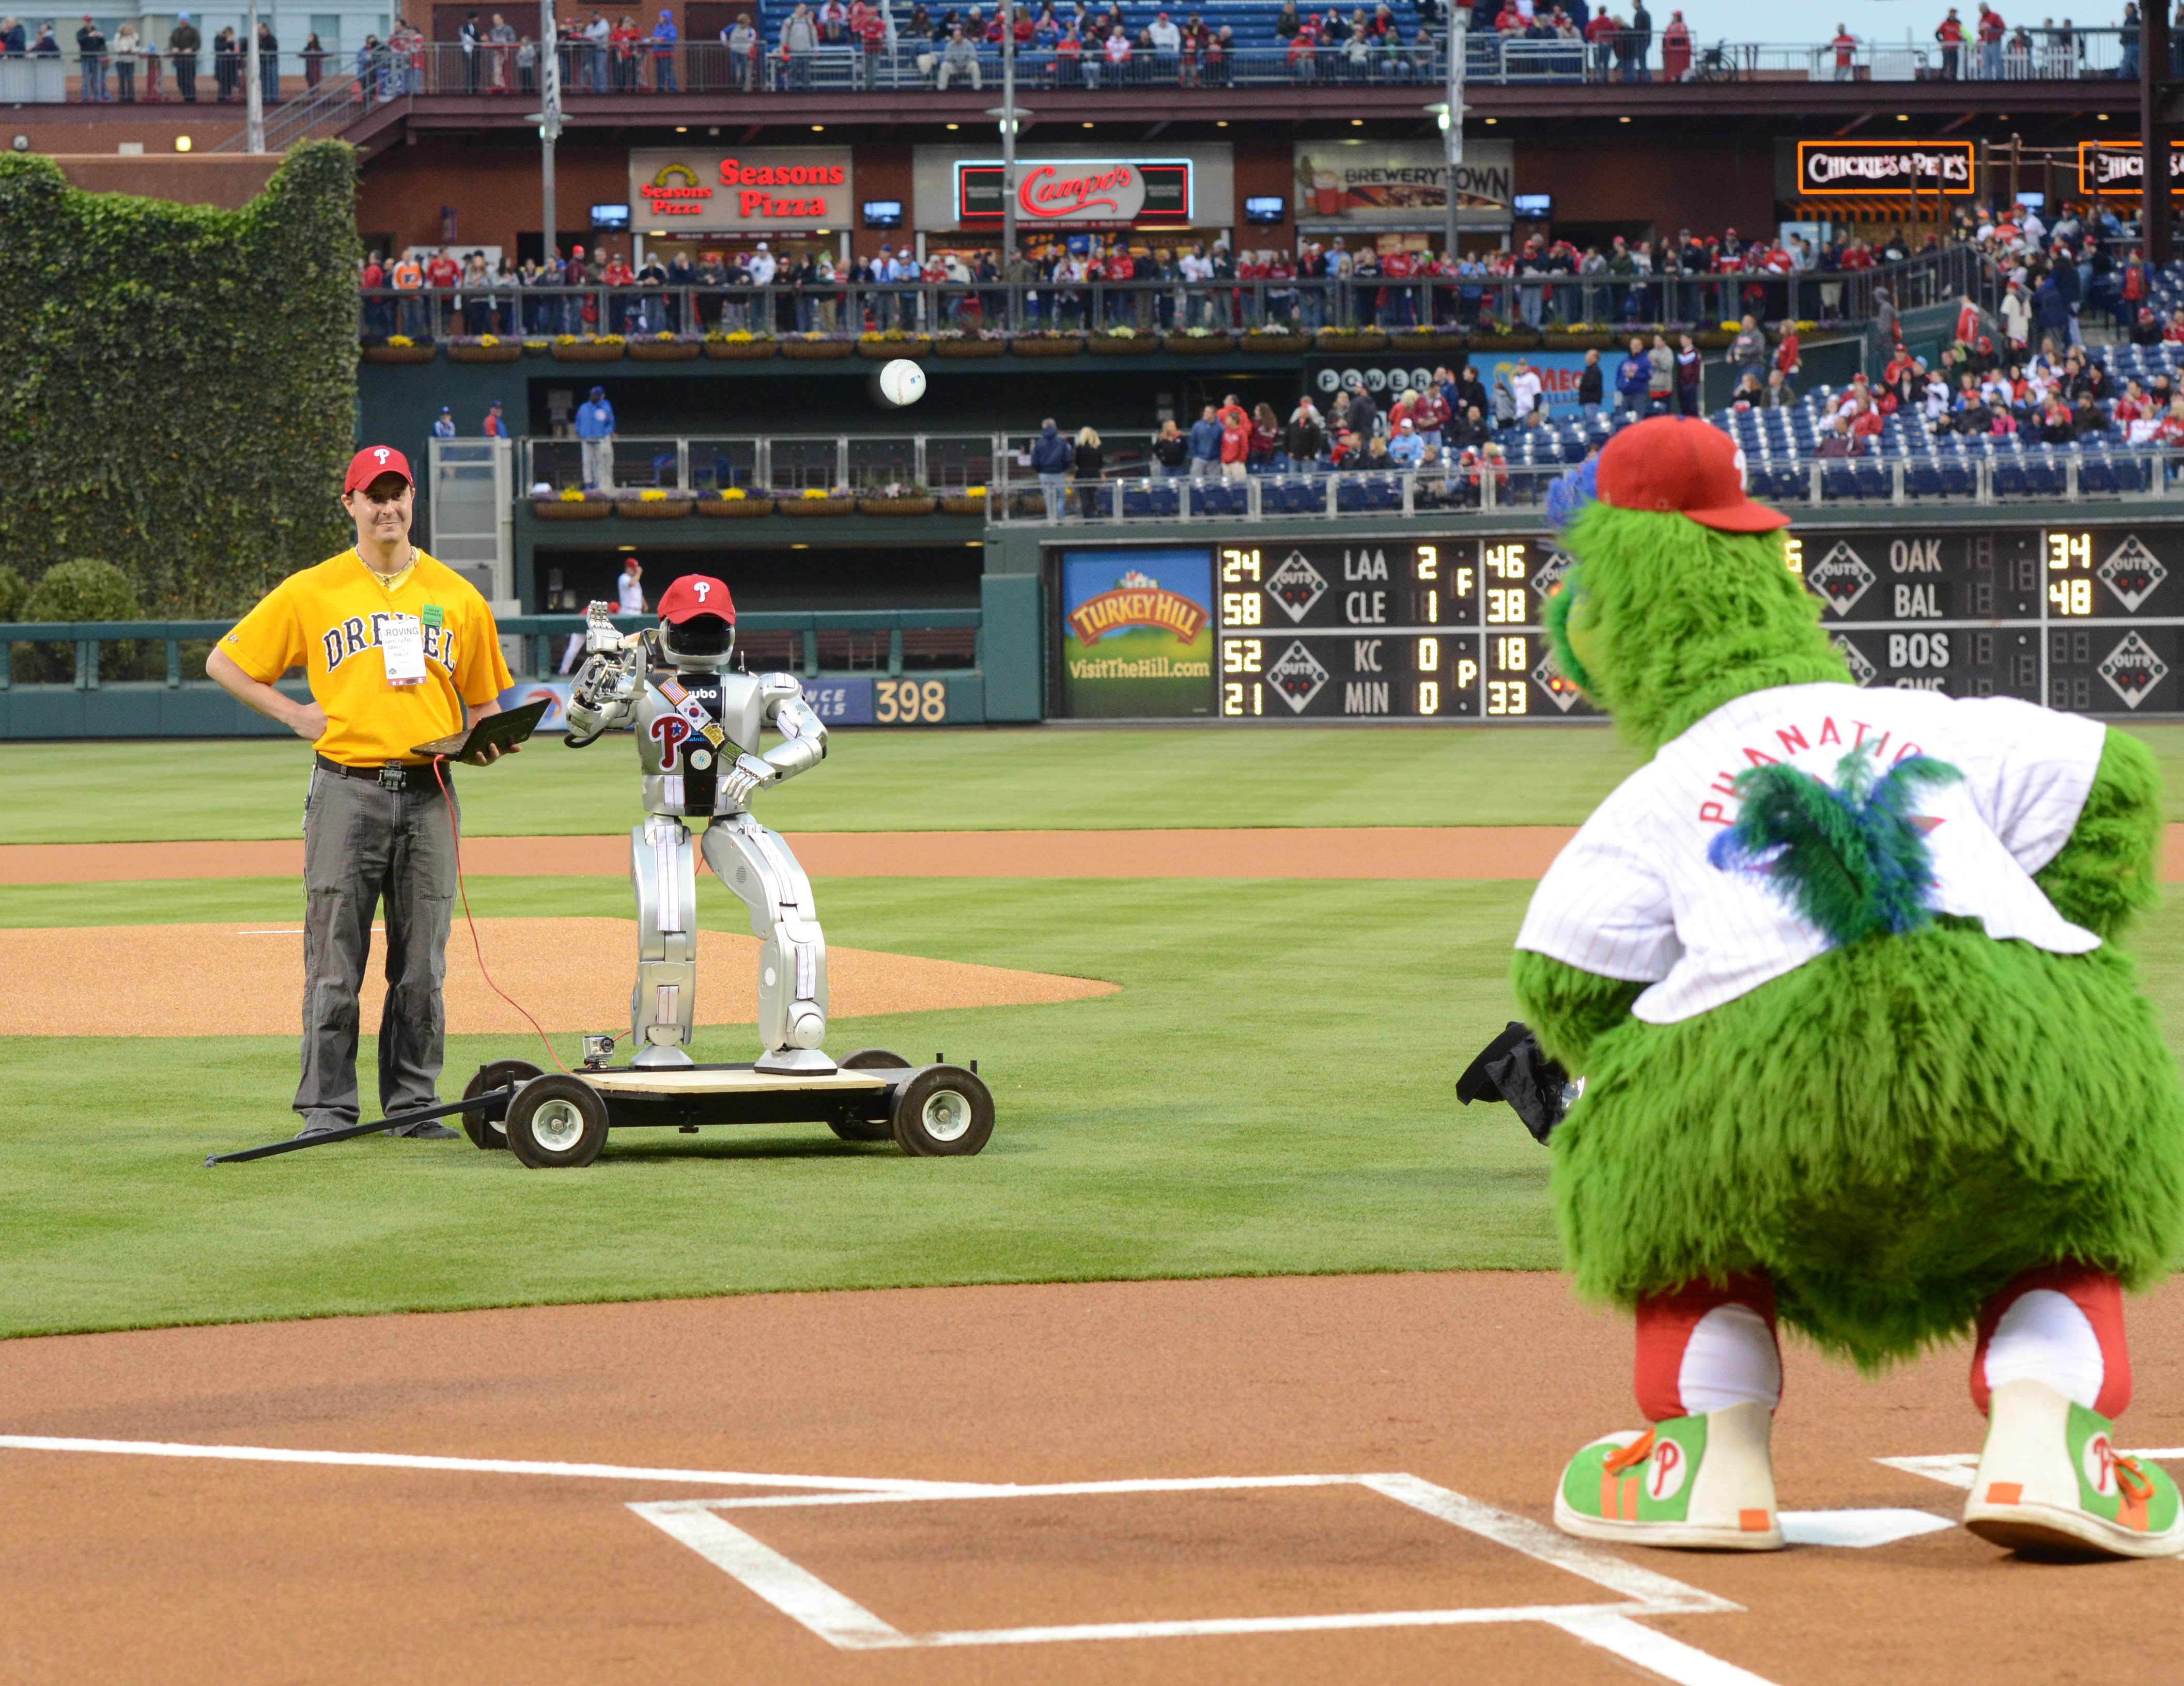
\includegraphics[width=1.0\columnwidth]{./pix/hubo-pitch.png}
  \caption{Hubo successfully throwing the first pitch at the second annual Philadelphia Science Festival event Science Night at the Ball Park on April 28th, 2012.  The game was between the Philadelphia Phillies and the Chicago Cubs and played at the Major League Baseball stadium Citizens Bank Park.  The Phillies won 5-2}
  \label{fig:hubo-throw}
\end{figure}


%The PhillieBot\footnote{PhillieBot Video: http://youtu.be/ShId-vZ-ZEY} made by the GRASP Lab at the University of Pennsylvania was the robot that threw the first pitch at the first annual Philadelphia Science Festival \textit{Science Night at the Ballpark} in 2011.  

Hubo was the first adult-size humanoid robot to throw the first pitch at a Major League baseball game.  
This document describes how this was done via the analyses and tests of three different approaches and the resulting final design.
Section~\ref{sec:background} gives a brief introduction to work already done in the field as well as states the requirements for the pitch.
Section~\ref{sec:methodology} describes the three different methods tested where:
Section~\ref{sec:sec:balance} discusses the balancing methods and criteria used.
Section~\ref{sec:sec:mocap} describes the kinematic mapping approach that uses a motion capture system to capture a human's throwing motion then mapping that to an adult-size humanoid robot.  
Section~\ref{sec:sec:srm} describes a fully automated approach that uses the sparse reachable map (SRM) to provide viable full body throwing trajectories to provide the end effector with the desired velocity\cite{dlofaro-srm}.
Section~\ref{sec:sec:keyframe} describes the final method explored which is based on key-frame trajectories.
Section~\ref{sec:comparison} Compares the tests and analyses of each of the methods.
Section~\ref{sec:finalDesign} describes in detail the remainder of the hurtals needed to be overcome to throw a successful pitch using the method chosen in Section~\ref{sec:comparison}.
Finally Section~\ref{sec:conclusion} gives final thoughts and possible improvements for future years.


%% remember robust and to say that you learned from upenns mistakes etc.